% Credits are indicated where needed. The general idea is based on a template by Vel (vel@LaTeXTemplates.com) and Frits Wenneker.

\documentclass[11pt, a4paper]{article} % General settings in the beginning (defines the document class of your paper)
% 11pt = is the font size
% A4 is the paper size
% “article” is your document class

%----------------------------------------------------------------------------------------
%	Packages
%----------------------------------------------------------------------------------------

% Necessary
\usepackage[german,english]{babel} % English and German language 
\usepackage{hyperref} % URL
\usepackage{subfig} %two figure
\usepackage{listings} % Insert code
\usepackage{float} % figure at the correct position
\usepackage{lipsum}
\usepackage{mwe}
\usepackage{booktabs} % Horizontal rules in tables 
% For generating tables, use “LaTeX” online generator (https://www.tablesgenerator.com)
\usepackage{comment} % Necessary to comment several paragraphs at once
\usepackage[utf8]{inputenc} % Required for international characters
\usepackage[T1]{fontenc} % Required for output font encoding for international characters

% Might be helpful
\usepackage{amsmath,amsfonts,amsthm} % Math packages which might be useful for equations
\usepackage{tikz} % For tikz figures (to draw arrow diagrams, see a guide how to use them)
\usepackage{tikz-cd}
\usetikzlibrary{positioning,arrows} % Adding libraries for arrows
\usetikzlibrary{decorations.pathreplacing} % Adding libraries for decorations and paths
\usepackage{tikzsymbols} % For amazing symbols ;) https://mirror.hmc.edu/ctan/graphics/pgf/contrib/tikzsymbols/tikzsymbols.pdf 
\usepackage{blindtext} % To add some blind text in your paper


%---------------------------------------------------------------------------------
% Additional settings
%---------------------------------------------------------------------------------

%---------------------------------------------------------------------------------
% Define your margins
\usepackage{geometry} % Necessary package for defining margins

\geometry{
	top=2cm, % Defines top margin
	bottom=2cm, % Defines bottom margin
	left=2.2cm, % Defines left margin
	right=2.2cm, % Defines right margin
	includehead, % Includes space for a header
	%includefoot, % Includes space for a footer
	%showframe, % Uncomment if you want to show how it looks on the page 
}

\setlength{\parindent}{15pt} % Adjust to set you indent globally 

%---------------------------------------------------------------------------------
% Define your spacing
\usepackage{setspace} % Required for spacing
% Two options:
\linespread{1.5}
%\onehalfspacing % one-half-spacing linespread

%----------------------------------------------------------------------------------------
% Define your fonts
\usepackage[T1]{fontenc} % Output font encoding for international characters
\usepackage[utf8]{inputenc} % Required for inputting international characters

\usepackage{XCharter} % Use the XCharter font


%---------------------------------------------------------------------------------
% Define your headers and footers

\usepackage{fancyhdr} % Package is needed to define header and footer
\pagestyle{fancy} % Allows you to customize the headers and footers

%\renewcommand{\sectionmark}[1]{\markboth{#1}{}} % Removes the section number from the header when \leftmark is used

% Headers
\lhead{} % Define left header
\chead{\textit{}} % Define center header - e.g. add your paper title
\rhead{} % Define right header

% Footers
\lfoot{} % Define left footer
\cfoot{\footnotesize \thepage} % Define center footer
\rfoot{ } % Define right footer

%---------------------------------------------------------------------------------
%	Add information on bibliography
\usepackage{natbib} % Use natbib for citing
\usepackage{har2nat} % Allows to use harvard package with natbib https://mirror.reismil.ch/CTAN/macros/latex/contrib/har2nat/har2nat.pdf

% For citing with natbib, you may want to use this reference sheet: 
% http://merkel.texture.rocks/Latex/natbib.php

%---------------------------------------------------------------------------------
% Add field for signature (Reference: https://tex.stackexchange.com/questions/35942/how-to-create-a-signature-date-page)
\newcommand{\signature}[2][5cm]{%
  \begin{tabular}{@{}p{#1}@{}}
    #2 \\[2\normalbaselineskip] \hrule \\[0pt]
    {\small \textit{Signature}} \\[2\normalbaselineskip] \hrule \\[0pt]
    {\small \textit{Place, Date}}
  \end{tabular}
}
%---------------------------------------------------------------------------------
%	General information
%---------------------------------------------------------------------------------
\title{Deep Learning Report} % Adds your title
%\author
%{
%    \name{Alfons Hwu} % Add your first and last name
%    %\thanks{} % Adds a footnote to your title
%    \\
%    \institution{0416324, Dept of Computer Science NCTU} % Adds your institution
%}



%---------------------------------------------------------------------------------
%	Define what’s in your document
%---------------------------------------------------------------------------------
\begin{document}


% If you want a cover page, uncomment "%---------------------------------------------------------------------------------
% Cover page
%---------------------------------------------------------------------------------

% Here are more templates for other cover pages: https://www.latextemplates.com/cat/title-pages

% This example is based on this cover page example: https://www.latextemplates.com/template/academic-title-page

\begin{titlepage} % Starts new environment where the page number is not displayed and the count starts at 1 for the next page

%------------------------------------------------
%	Institutional information
%------------------------------------------------
	
\begin{minipage}{0.4\textwidth} % Begins new environment (like a text box)
    \begin{flushleft} % Sets environment on the left side of the paper
    \large
    National Chiao Tung University\\ % Add your institution
    Spring 2019 \\ % Add term
    Deep Learning \\ % Add course title
    Instructor: Jen-Tsung Chien\\ % Add instructor/supervisor name 
    \end{flushleft}
\end{minipage}
	
\vspace*{2in} % Adds some space in-between
	
\center % Centre everything on the page

%------------------------------------------------
%	Main part
%------------------------------------------------
	
{\huge\bfseries Deep Learning HW2 Report}\\[0.4cm] % Add your paper title {\large\today}\\[0.4cm] % Add date (current day)
Alfons Hwu \\ % Add your name
Student ID: 0416324\\
\vfill % Adds additional space

%------------------------------------------------
%	General information about the author
%------------------------------------------------

\vfill % Adds additional space

alfons.cs04@g2.nctu.edu.tw \\ % Add your contact info
Dept of Computer Science \\ % Add info about your program
Writing with \LaTeX  on Overleaf

\vfill % Adds additional space

%------------------------------------------------
%	Word count
%------------------------------------------------

\vfill % Adds additional space
	
\end{titlepage}" and uncomment "\begin{comment}" and "\end{comment}" to comment the following lines
%---------------------------------------------------------------------------------
% Cover page
%---------------------------------------------------------------------------------

% Here are more templates for other cover pages: https://www.latextemplates.com/cat/title-pages

% This example is based on this cover page example: https://www.latextemplates.com/template/academic-title-page

\begin{titlepage} % Starts new environment where the page number is not displayed and the count starts at 1 for the next page

%------------------------------------------------
%	Institutional information
%------------------------------------------------
	
\begin{minipage}{0.4\textwidth} % Begins new environment (like a text box)
    \begin{flushleft} % Sets environment on the left side of the paper
    \large
    National Chiao Tung University\\ % Add your institution
    Spring 2019 \\ % Add term
    Deep Learning \\ % Add course title
    Instructor: Jen-Tsung Chien\\ % Add instructor/supervisor name 
    \end{flushleft}
\end{minipage}
	
\vspace*{2in} % Adds some space in-between
	
\center % Centre everything on the page

%------------------------------------------------
%	Main part
%------------------------------------------------
	
{\huge\bfseries Deep Learning HW2 Report}\\[0.4cm] % Add your paper title {\large\today}\\[0.4cm] % Add date (current day)
Alfons Hwu \\ % Add your name
Student ID: 0416324\\
\vfill % Adds additional space

%------------------------------------------------
%	General information about the author
%------------------------------------------------

\vfill % Adds additional space

alfons.cs04@g2.nctu.edu.tw \\ % Add your contact info
Dept of Computer Science \\ % Add info about your program
Writing with \LaTeX  on Overleaf

\vfill % Adds additional space

%------------------------------------------------
%	Word count
%------------------------------------------------

\vfill % Adds additional space
	
\end{titlepage}

\date{May 31, 2019}
\begin{comment}
\end{comment}
\maketitle{} %Print your title, author name and date; comment if you want a cover page 

%----------------------------------------------------------------------------------------
% Introduction
%----------------------------------------------------------------------------------------
\setcounter{page}{1} % Sets counter of page to 1

\section{Self-designed VAE for unsupervised learning} % Add a section title
\subsection{Preprocessing and architecture} % Section check OK 20190502
In the preprocessing part, I merely resize the image to 64 x 64 . No gray scale transformation nor random crop and(or) rotate to form data augmentation.
\\ For the architecture, I choose CNN for VAE rather than DNN since it fits better for image processing.
(In DNN, the network was not able to process the color channels separately, resulting in an average RGB scale of a grey image)
\\ Use some convolution layer to extracting the image characteristics, then DNN to calculate the mean and variance and finally reparameterize by shifting the  $N~(0, 1)$ to approach $N~(\mu \epsilon)$
\\ Referencing to \url{}
\begin{lstlisting}[language = python]
class VAE(nn.Module):
    def __init__(self, image_channels = 3, h_dim = 1024, z_dim = 32):
        super(VAE, self).__init__()
        self.encoder = nn.Sequential(
            nn.Conv2d(image_channels, 32, kernel_size = 4, stride = 2),
            nn.ReLU(),
            nn.Conv2d(32, 64, kernel_size = 4, stride = 2),
            nn.ReLU(),
            nn.Conv2d(64, 128, kernel_size = 4, stride = 2),
            nn.ReLU(),
            nn.Conv2d(128, 256, kernel_size = 4, stride = 2),
            nn.ReLU(),
            flatten()
        )

        self.fc1 = nn.Linear(h_dim, z_dim)
        self.fc2 = nn.Linear(h_dim, z_dim)
        self.fc3 = nn.Linear(z_dim, h_dim)

        self.decoder = nn.Sequential(
            unflatten(),
            nn.ConvTranspose2d(h_dim, 128, kernel_size = 5, stride = 2),
            nn.ReLU(),
            nn.ConvTranspose2d(128, 64, kernel_size = 5, stride = 2),
            nn.ReLU(),
            nn.ConvTranspose2d(64, 32, kernel_size = 6, stride = 2),
            nn.ReLU(),
            nn.ConvTranspose2d(32, image_channels, kernel_size = 6, stride = 2),
            nn.ReLU()
        )
\end{lstlisting}

\subsection{CNN architecture explanation and performance evaluation} % Add a subsection
\subsubsection{Architecture}
\\ Main architecture is similar to that of famous VGG16, yet concerning the hardware limitation , I condense them into only 8 convolutional layers and two linear(normal dnn) layer in the end.   The following figure show the VGG16 architecture.
\\ \small{With original architecture layer representing in list, M represents the maxpool layer and number is the channel size.}
\\ VGG16 = [64, 64, 'M', 128, 128, 'M', 256, 256, 256, 'M', 512, 512, 512, 'M', 512, 512, 512, 'M']
\\ And here is my condensed version
\\ VGG16-small = [8, 'M', 16, 'M', 32, 'M', 64, 'M']
\\ The filter size is reduced to 1/8 in total and for each stacked layer between two maxpool layer, I extract one from them since it is enough to represent the overall architecture, larger kernel size will only increase the computational complexity. 
\\ After that, data are fed into the classification layer, the output size of image will changed to 7 x 7 x 64. flatten to the dnn for the final classification.
\\ The following is the architecture of classification layers, ReLU is applied here since it first prevents gradient vanishing, second it provides sparsity with an eye to preventing overfitting (and also reduce computational workload), last but not least, it bears a resemblance to \textbf{all or none law} similar to that of nature species. Drop out is used to prevent overfitting and finally the linear output of classification result.
\begin{lstlisting}[language = python]
self.classifier = nn.Sequential(
                nn.Linear(64 * 7 * 7, linear_size),
                nn.ReLU(True),
                nn.Dropout(),
                nn.Linear(linear_size, len(classes)),
                )
\end{lstlisting}
\\ Compare my CNN with original VGG16,   
\\ Actually, the original VGG16 did perform a bit better but both of the test acc get stuck (overfitting), hence the depth size is not the main concern and further tuning will be discussed later(Due to VRAM limitation, original vgg16 can only be fitted with 40 images/batch)
\begin{figure}[H]
  \centering
  \subfloat[Original VGG16]{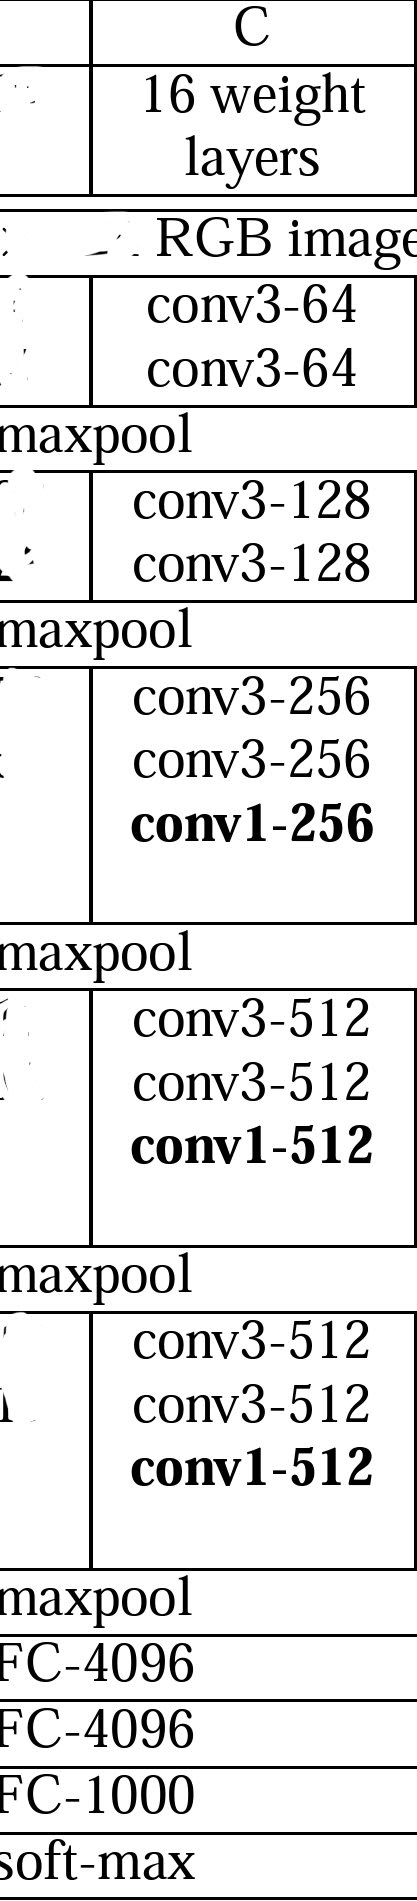
\includegraphics[scale = 0.1]{HW2/arch_diagram/orig.jpg}\label{fig:f1}}
  \hfill
  \subfloat[My own VGG]{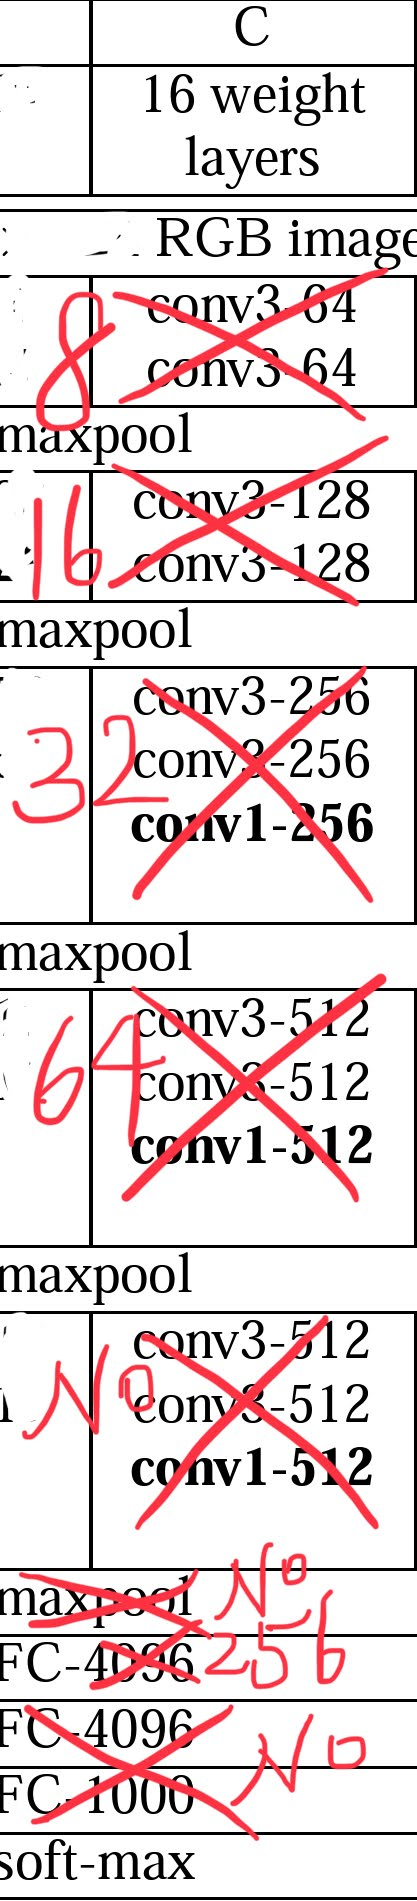
\includegraphics[scale = 0.1]{HW2/arch_diagram/my.jpg}\label{fig:f2}}
  \caption{VGG comparison}
\end{figure}

\subsubsection{The learning curve vs kernel and stride size}
{\Large Experiments to check the effect of kernel and stride size on result}
\\ First we compare the effect of kernel size, both of which use the same stride, optimizer, lr and batch size.
We are able to clearily see that the small kernel size performed slightly better than large one. In my perspective, larger convolutional kernel probably will mix more pixel around the center pixel, causing more noise in training.
\\ (Reference: \url{https://zhuanlan.zhihu.com/p/41423739}), in this link, author mentioned about "receptive" filed, that is stacked some of the small convolutional layer may not only better preserve the properties of original image(less "mixing" effect) but also cost less parameters during computation. 

\begin{figure}[H]
  \centering
  \subfloat[Kernel size 3]{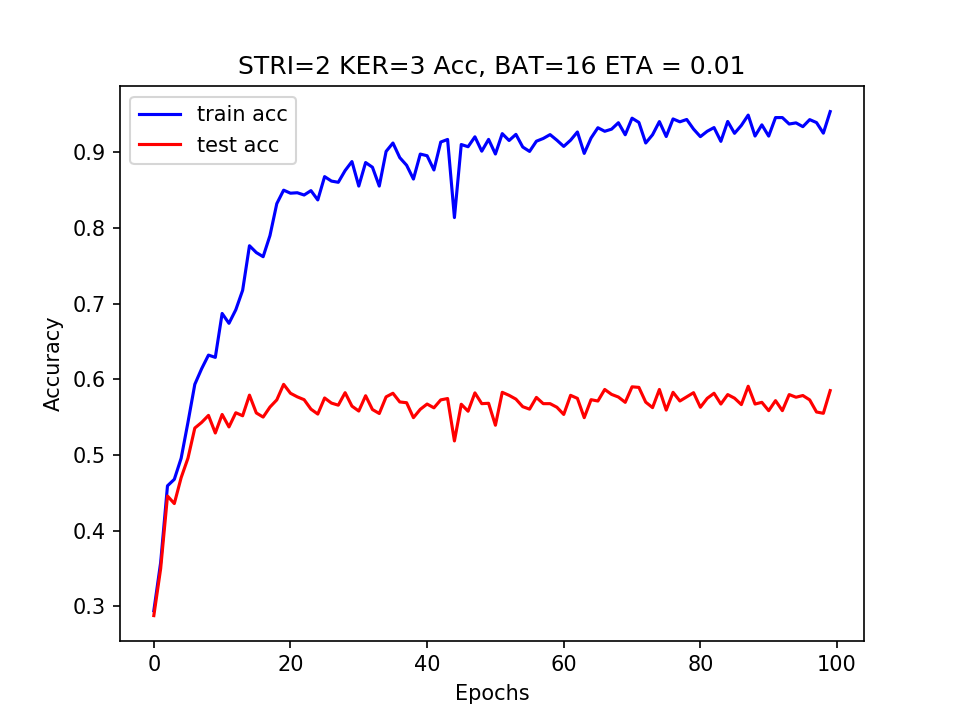
\includegraphics[scale = 0.5]{HW2/cmp_kernel/ker_3_acc.png}\label{fig:f1}}
  \hfill
  \subfloat[Kernel size 5]{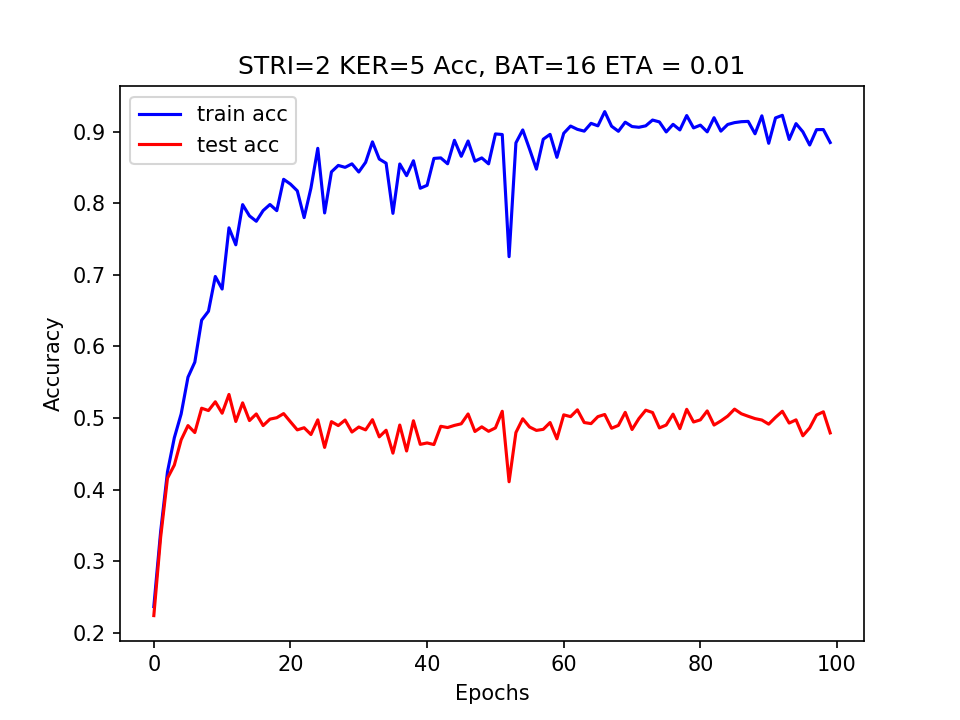
\includegraphics[scale = 0.5]{HW2/cmp_kernel/ker_5_acc.png}\label{fig:f1}}
  \caption{Convolutional layer kernel size comparison}
\end{figure}
\\ Then we compare the effect of stride size, both of which use the same kernel size, optimizer, lr and batch size.
We can see that the small stride performed slightly better than large one. In my perspective, the higher the stride size is, the less image detail it will be filtered out(or preserved) by the kernel. 
\begin{figure}[H]
  \centering
  \subfloat[Stride size 1]{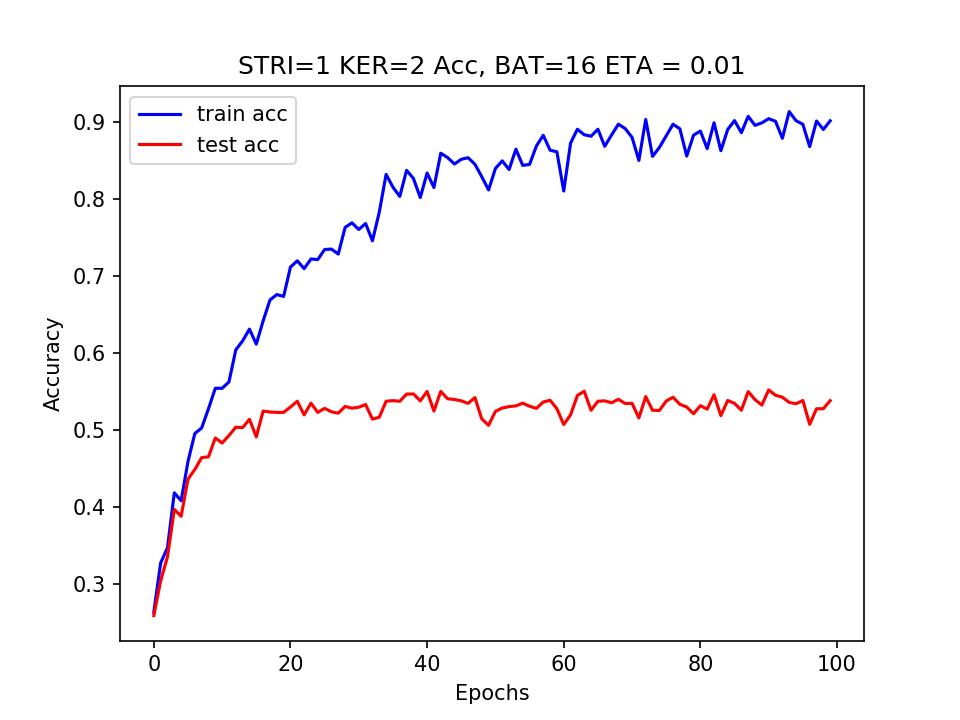
\includegraphics[scale = 0.5]{HW2/cmp_stride/stri_1_acc.png}\label{fig:f1}}
  \hfill
  \subfloat[Stride size 3]{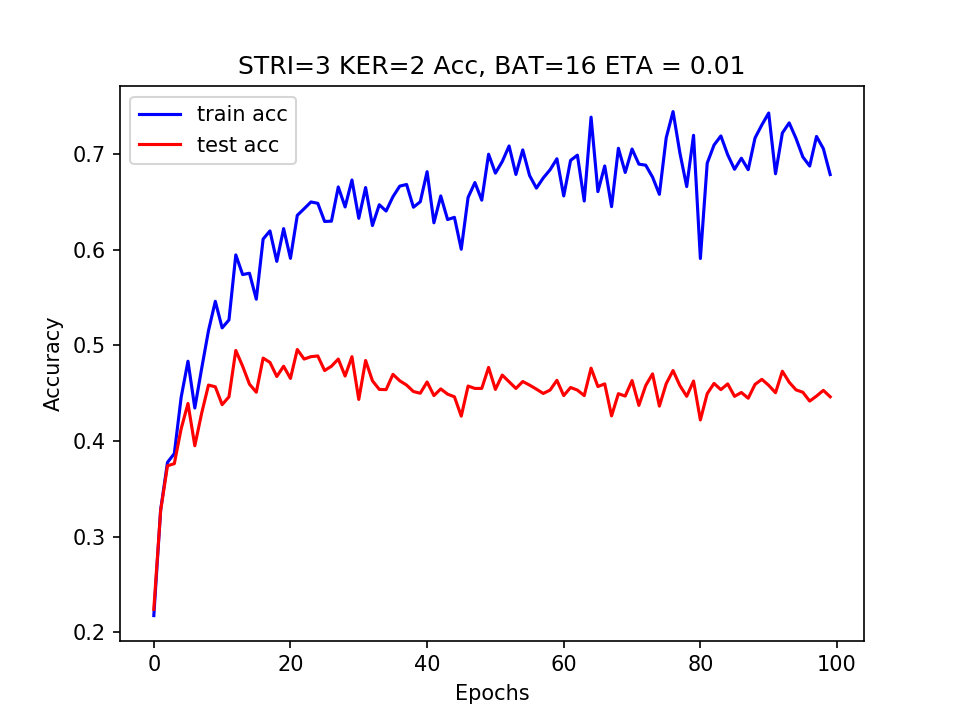
\includegraphics[scale = 0.5]{HW2/cmp_stride/stri_3_acc.png}\label{fig:f1}}
  \caption{Convolutional layer stride size comparison}
\end{figure}
{\Large Conclusion}
\\ Kernel size 3 and stride 2(no overlapping for maxpool size 2) will be enough. \newline \break
{\Large Experiments to find the best optimizing method}
\\ In this project, I have tried using three method to tune my model.
\\ First, by using SGD with momentum and L2 penalty to prevent overfitting
\\ Second, by using adam L2 penalty to prevent overfitting
\begin{figure}[H]
    \centering
    \subfloat[SGD with momentum and L2 penalty]{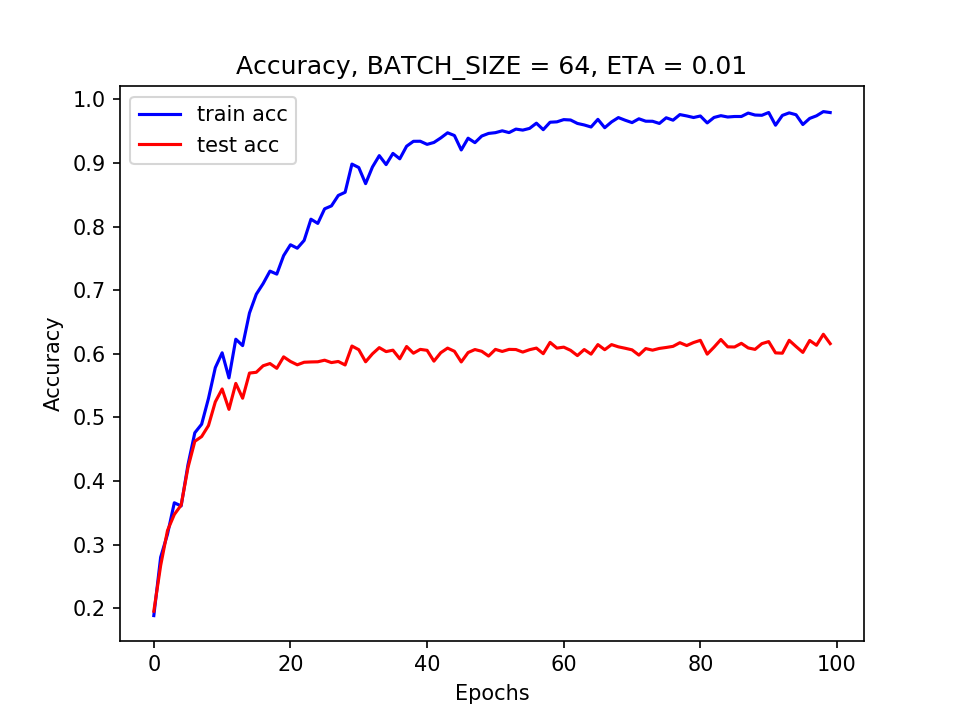
\includegraphics[scale = 0.5]{HW2/cmp_method/sgd.png}}
    \hfill
    \subfloat[Adam with L2 penalty]{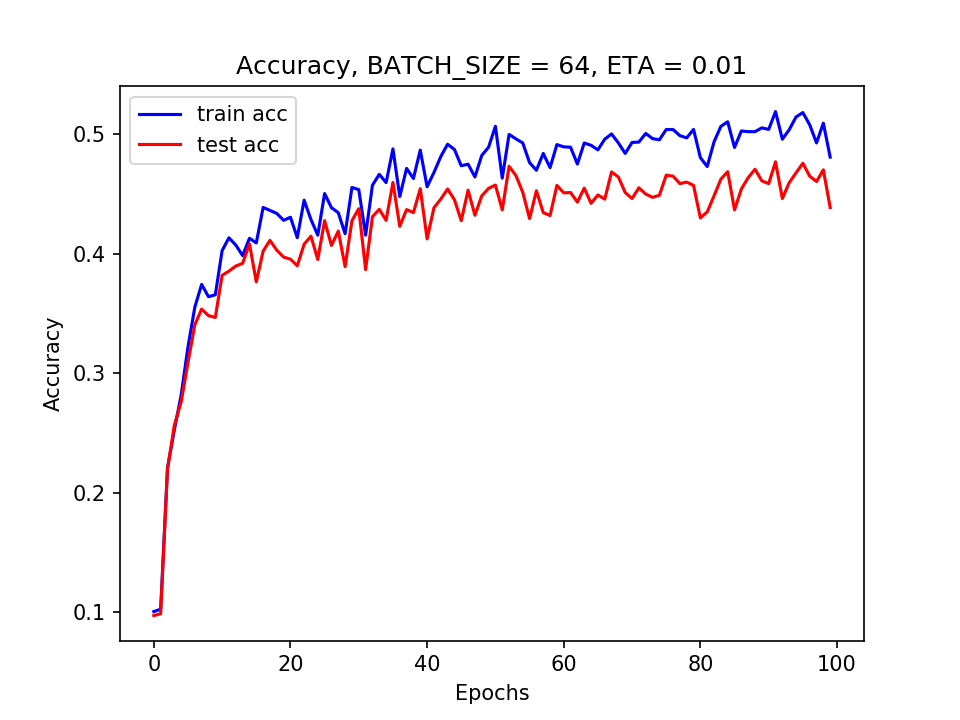
\includegraphics[scale = 0.5]{HW2/cmp_method/adam.png}}
    \caption{Optimizing method comparison}
    \label{fig:my_label}
\end{figure}
\\ We can see that the accuracy of testing set in SGD with momentum got stuck in about 30th epoch. Although the curve of adam kept damping, it did not stuck as severe as SGD with momentum. \newline \break 
{\Large Conclusion}
\\ Extend the epoch to see if one outperformed the other.
\\ Finally the \texttt{batch\_size 128, adam optimizer(initial learning rate 5e-4), stride\_size 2} performs the best and here is the overall best result. 
\subsection{The accuracy results and related discussion}
\begin{figure}[H]
    \centering
    \subfloat[Accuracy by class]{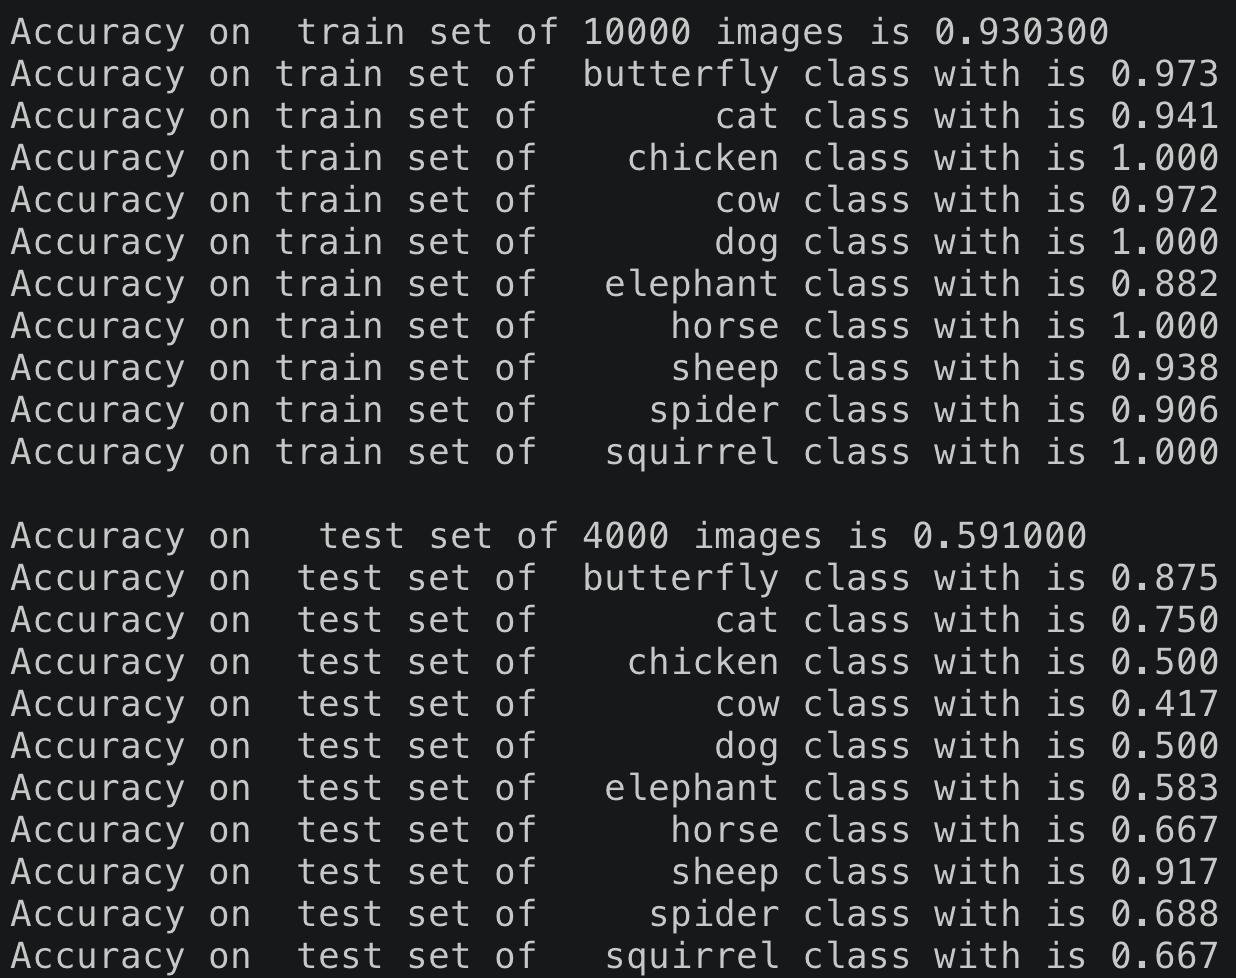
\includegraphics[scale = 0.5]{HW2/cnn_result/class_acc_1.png}}
    \hfill
    \subfloat[Accuracy curve]{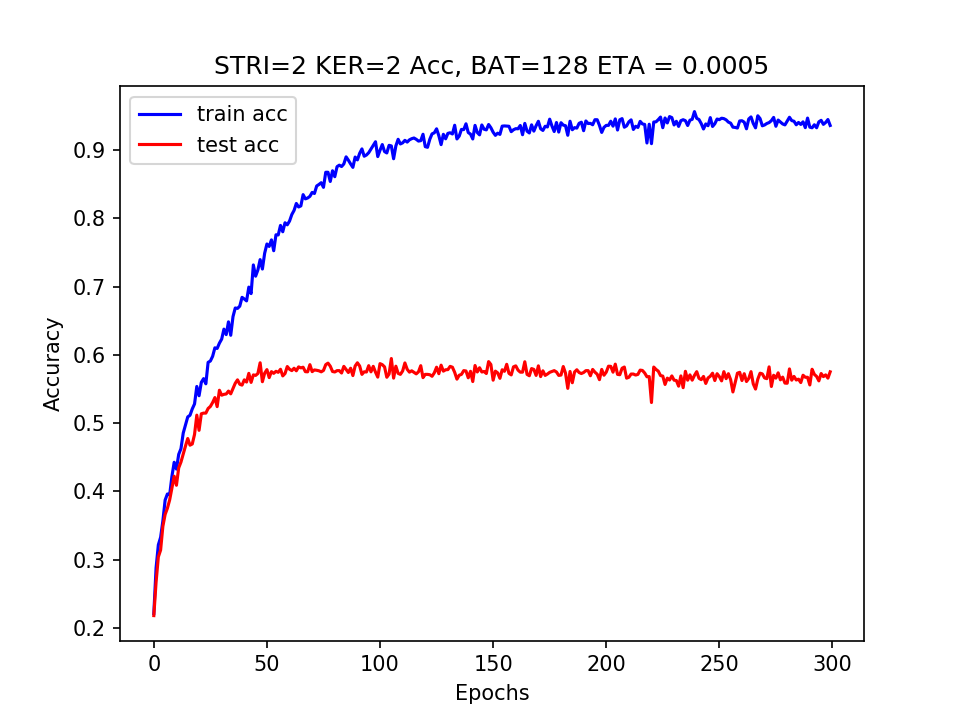
\includegraphics[scale = 0.5]{HW2/cnn_result/acc.png}}
    \hfill
    \subfloat[Loss curve]{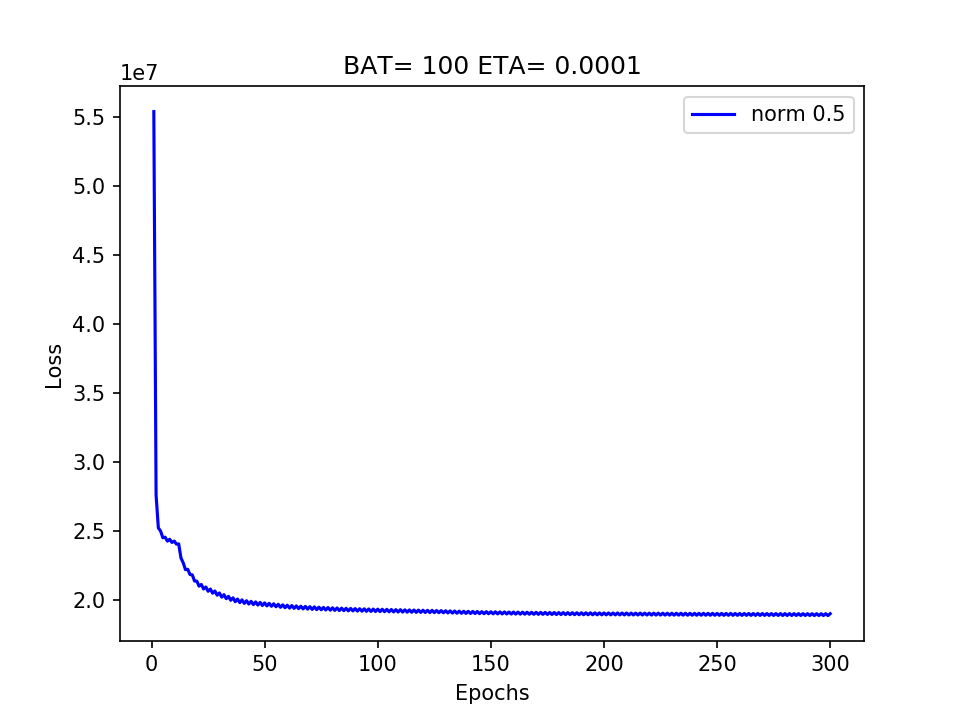
\includegraphics[scale = 0.5]{HW2/cnn_result/lc.png}}
    \hfill
    \caption{Overall best result}
    \label{fig:my_label}
\end{figure}
%\\ Reason for class \texttt{class class class} perform well mainly lies in
\\ Following are the example of incorrectly-classfied images {\small(the filename format are used to represent the incorrectly format: label\_predicted\_errorcount.png)}
\begin{figure}[H]
    \centering
    \subfloat[Filename format]{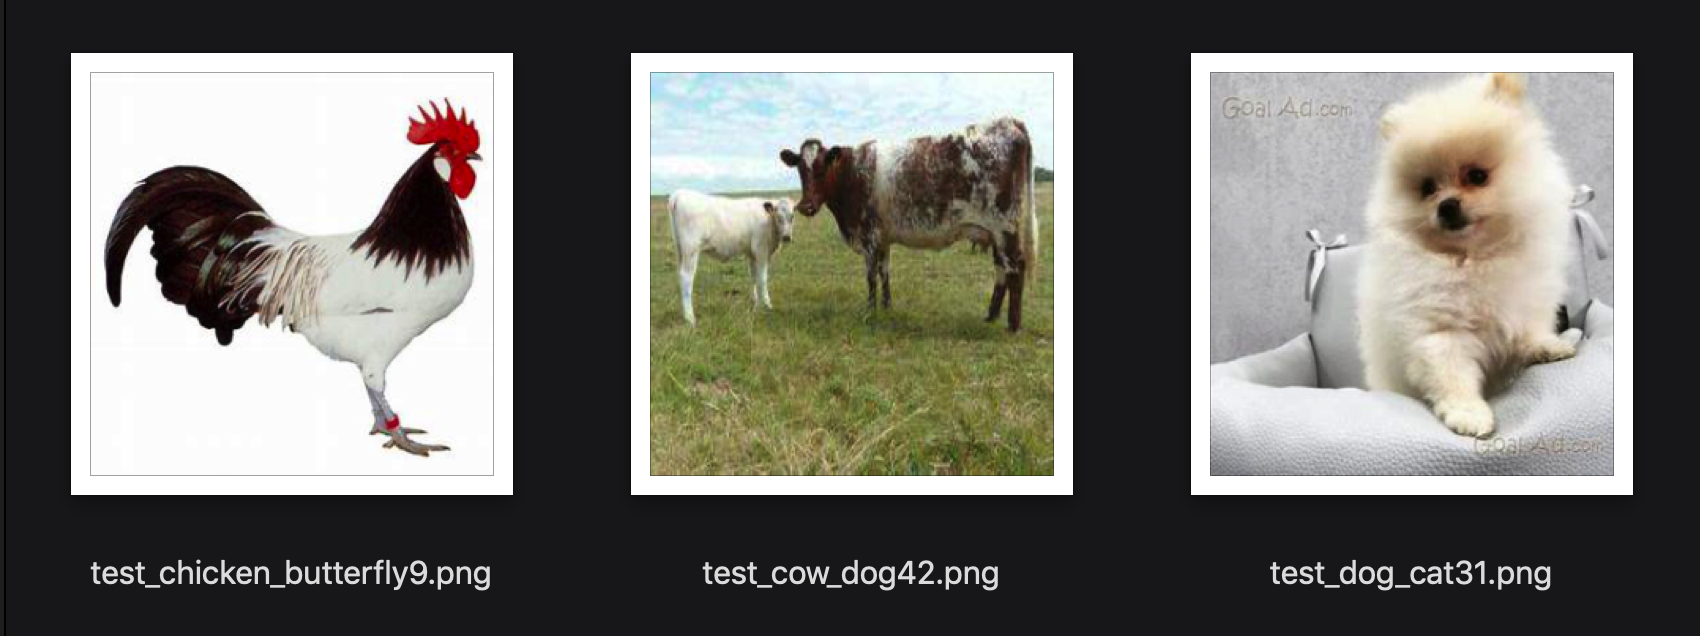
\includegraphics[scale = 0.5]{HW2/wrong_classified/name.png}}
    \hfill
    \subfloat[Label chicken, predict butterfly]{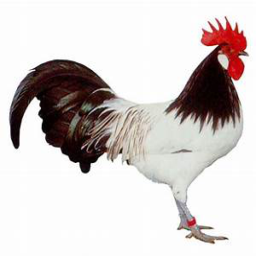
\includegraphics[scale = 0.4]{HW2/wrong_classified/test_chicken_butterfly9.png}}
    \hfill
    \subfloat[Label cow, predict dog]{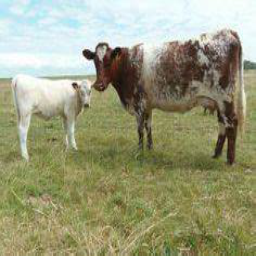
\includegraphics[scale = 0.4]{HW2/wrong_classified/test_cow_dog42.png}}
    \hfill
    \subfloat[Label dog, predict cat]{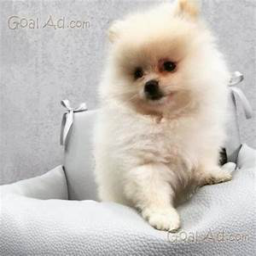
\includegraphics[scale = 0.4]{HW2/wrong_classified/test_dog_cat31.png}}
    \hfill
    \caption{Incorrectly-classified images}
    \label{fig:my_label}
\end{figure}
{\Large \\ Further discussions (My deductions)}
\\ Reason for class \texttt{chicken cow dog} perform poor mainly lies in
\begin{itemize}
    \item Chicken: The side-view of chicken may bear resemblance butterfly.
    \item Cow: The side-view of cow may bear resemblance to either dog or cat. 
    \item Dog: The front and side view of dog may bear resemblance to cat, since in Taxonomy
    they both lie under Animalia/Mammalia/Carnivora 
\end{itemize}

\section{Self-designed RNN for NLP}
\subsection{Conventional RNN}
\subsubsection{Preprocessing}
In the preprocessing part, I crop (or padding) the sentence to make each of them in the length of 10 and each word corresponding to the vector length of 10 as well.
Finally, each sentence can be represented to the matrix size of 10x10.
The preprocessing code is here \url{https://github.com/Alfons0329/DL_Spring_2019/blob/master/HW2/RNN/preprocessing_2.py}
\\ For example
\texttt{This is not an apple} in the embedding process, it will be converted to \texttt{This is not an apple XXX XXX XXX XXX XXX} since \texttt{XXX} is the 0th element in the while dictionary and thus being used for padding the sentence.
\\ And finally \texttt{1 2 3 4 5 0 0 0 0 0} and be converted to matrix representation of size 10 x 10 by the rule of word embedding.
\\ Reference tutorial: \url{https://pytorch.org/tutorials/beginner/nlp/word_embeddings_tutorial.html}
\subsubsection{Architecture explanation}
\\ The RNN architecture is as follows: The input size is a 10-dimension wordvector and time step is set as 10 as we output the binary classification result based on the sentence of length 10.

\begin{lstlisting}[language = python]
self.rnn = nn.RNN(
                input_size = 10,
                hidden_size = N_HID_SIZE,
                num_layers = 1,
                dropout = 0.5,
                batch_first = True,
                bidirectional = False
                )
self.classifier = nn.Sequential(
                nn.Linear(N_HID_SIZE, 1),
                nn.Sigmoid(),
                )

inputs = inputs.view(N_BATCH_SIZE, N_RNN_STEP, N_VEC_WORD) \# reshape
\end{lstlisting}

\subsubsection{Results }

\begin{figure}[H]
    \centering
    \subfloat[Accuracy curve(adam)]{\includegraphics[scale = 0.5]{HW2/rnn_result/adam_1_acc.png}}
    \hfill
    \subfloat[Loss curve(adam)]{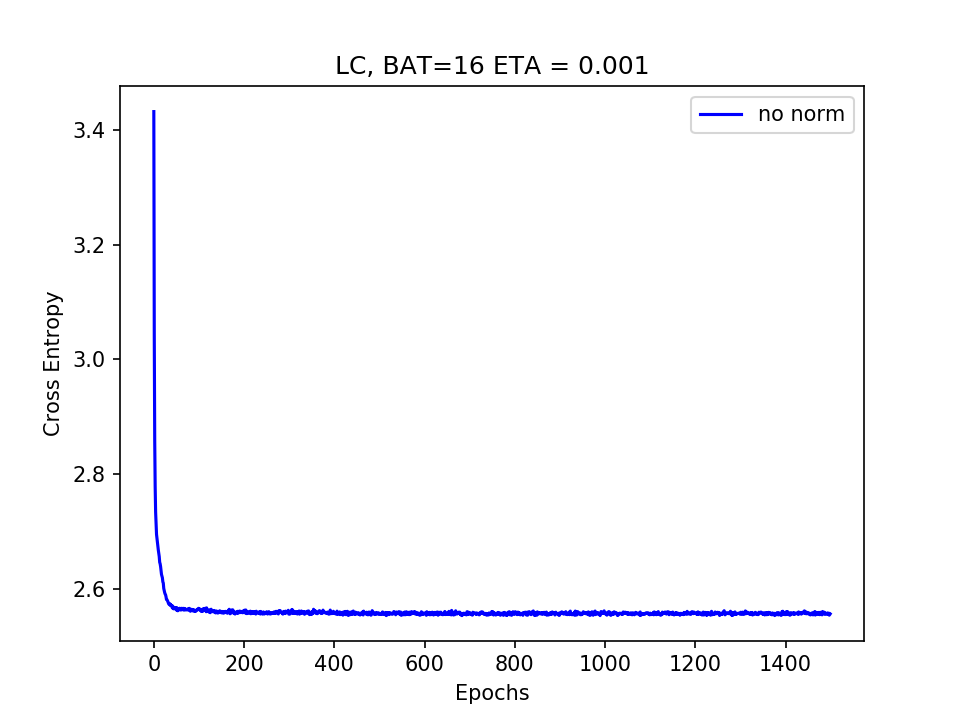
\includegraphics[scale = 0.5]{HW2/rnn_result/adam_1_lc.png}}
    \hfill
    \subfloat[Accuracy curve(adam)]{\includegraphics[scale = 0.5]{HW2/rnn_result/adam_2_acc.png}}
    \hfill
    \subfloat[Loss curve(adam)]{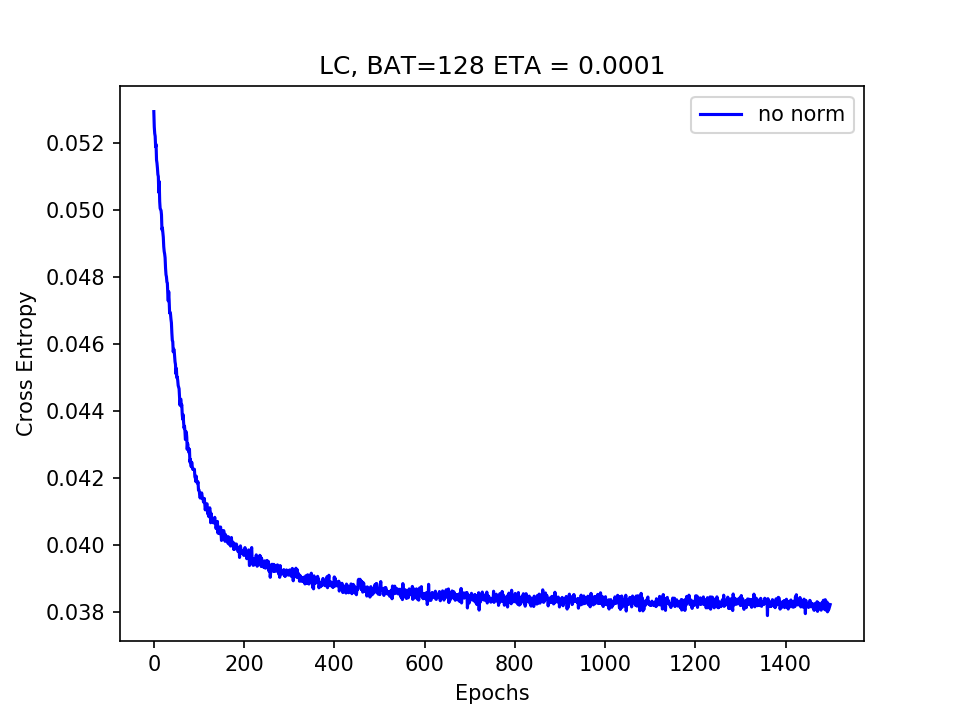
\includegraphics[scale = 0.5]{HW2/rnn_result/adam_2_lc.png}}
    \hfill
    \subfloat[Accuracy curve(sgd)]{\includegraphics[scale = 0.5]{HW2/rnn_result/sgd_1_acc.png}}
    \hfill
    \subfloat[Loss curve(sgd)]{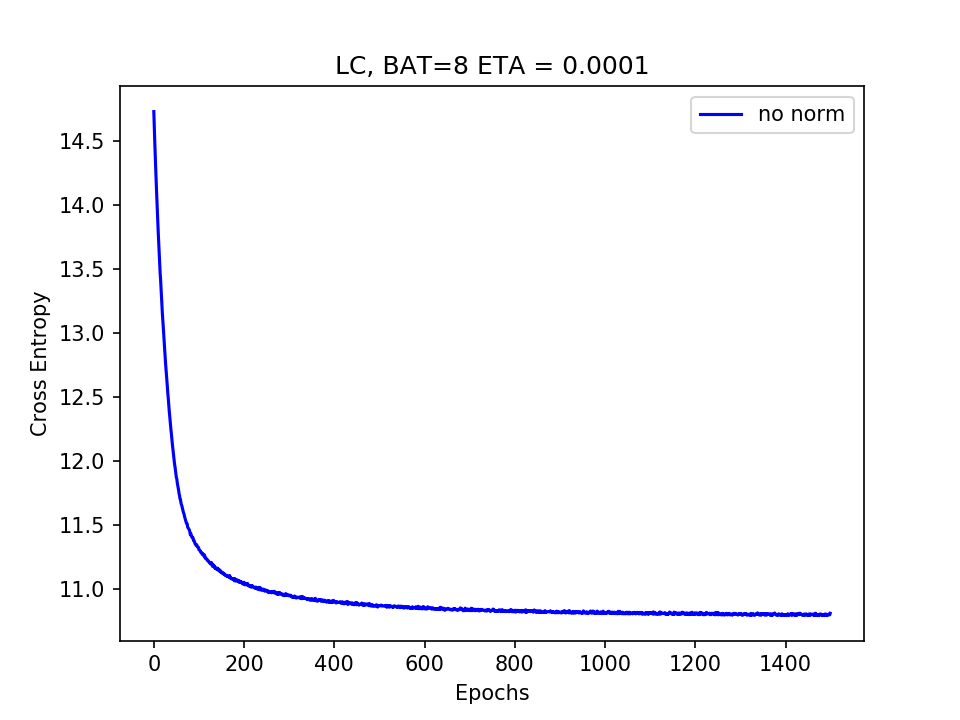
\includegraphics[scale = 0.5]{HW2/rnn_result/sgd_1_lc.png}}
    \caption{RNN results}
    \label{fig:my_label}
\end{figure}
\subsubsection{LSTM results vs RNN results}
\begin{figure}[H]
    \centering
    \subfloat[Accuracy curve of LSTM(adam)]{\includegraphics[scale = 0.5]{HW2/lstm_result/adam_1_acc.png}}
    \hfill
    \subfloat[Accuracy curve of RNN(adam)]{\includegraphics[scale = 0.5]{HW2/rnn_result/adam_1_acc.png}}
    \hfill
    \subfloat[Accuracy curve of LSTM(adam)]{\includegraphics[scale = 0.5]{HW2/lstm_result/adam_2_acc.png}}
    \hfill
    \subfloat[Accuracy curve of RNN(adam)]{\includegraphics[scale = 0.5]{HW2/rnn_result/adam_2_acc.png}}
    \hfill
    \subfloat[Accuracy curve of LSTM(sgd)]{\includegraphics[scale = 0.5]{HW2/lstm_result/sgd_1_acc.png}}
    \hfill
    \subfloat[Accuracy curve of RNN(sgd)]{\includegraphics[scale = 0.5]{HW2/rnn_result/sgd_1_acc.png}}
    \caption{Accuracy comparison}
    \label{fig:my_label}
\end{figure}
\\ By merely changed the network from RNN to LSTM (all the rest are remain unchanged, including the optimization method).
\\ As the figures shown, RNN may suffer from the gradient vanishing/exploding in the latter epochs during training.

\subsection{Discussion: LSTM vs RNN}
\\ Reference \url{https://colah.github.io/posts/2015-08-Understanding-LSTMs/}
\\ In theory, RNNs are absolutely capable of handling such “long-term dependencies.” A human could carefully pick parameters for them to solve toy problems of this form. Sadly, in practice, RNNs don’t seem to be able to learn them. The problem was explored in depth by Hochreiter (1991) [German] and Bengio, et al. (1994), who found some pretty fundamental reasons why it might be difficult.
\subsubsection{Gradient vanishing and exploding}
\\ The back propogation is defined as: $w^{t+1} = w^{t} - \eta\Delta E(w^{t})$ 
\\ The gradients coming from the deeper layers have to go through continuous matrix multiplications because of the the chain rule, and as they approach the earlier layers, if they have small values (<1), they shrink exponentially until they vanish and make it impossible for the model to learn , this is the \textbf{vanishing gradient problem}. While on the other hand if they have large values (>1) they get larger and eventually blow up and crash the model, this is the \textbf{exploding gradient problem}
\\
\\
\\
\\ {\Large Conclusion: The advantage of LSTM}
\\ The memory cell remembers the first input as long as the forget gate is open and the input gate is closed while output gate provides finer control to switch the output layer on or off without altering the cell contents, thus solve the gradient vanishing/exploding problem.
\end{document}